%----------------------------------------------------------------------------------------
%   PHẦN 4: KẾT QUẢ THỰC NGHIỆM
%----------------------------------------------------------------------------------------
\section{Kết quả thực nghiệm}

\begin{frame}{Môi trường thực nghiệm}
    \begin{table}
        \centering
        \begin{tabular}{|l|l|}
            \hline
            \textbf{Thành phần} & \textbf{Thông số} \\
            \hline
            \multicolumn{2}{|c|}{\textit{Huấn luyện (Kaggle Cloud)}} \\
            \hline
            GPU & NVIDIA Tesla P100-PCIE (16GB) \\
            \hline
            CPU & 4 Logical Cores \\
            \hline
            RAM & 31.35 GB \\
            \hline
            \multicolumn{2}{|c|}{\textit{Inference (Local)}} \\
            \hline
            GPU & RTX 4060 / RTX 2050 \\
            \hline
            Framework & PyTorch 2.0, CUDA 12.4 \\
            \hline
        \end{tabular}
        \caption{Cấu hình môi trường thực nghiệm}
    \end{table}
\end{frame}

%--- SO SÁNH 3 MÔ HÌNH ---
\begin{frame}{So sánh kết quả huấn luyện 3 mô hình}
    \begin{table}
        \centering
        \small
        \begin{tabular}{|l|c|c|c|c|}
            \hline
            \textbf{Mô hình} & \textbf{Precision} & \textbf{Recall} & \textbf{mAP@50} & \textbf{mAP@50-95} \\
            \hline
            \textbf{Model 1: Phát hiện xe} & 87.2\% & 78.1\% & 86.1\% & 70.4\% \\
            \textit{(YOLOv8n, 5 lớp)} & & & & \\
            \hline
            \textbf{Model 2: Phát hiện biển} & \textbf{99.97\%} & \textbf{99.86\%} & \textbf{99.50\%} & \textbf{81.90\%} \\
            \textit{(YOLOv8n, 1 lớp)} & & & & \\
            \hline
            \textbf{Mô hình tích hợp} & 84.7\% & 71.6\% & 78.5\% & 62.3\% \\
            \textit{(YOLOv8n, 6 lớp)} & & & & \\
            \hline
        \end{tabular}
        \caption{So sánh kết quả 3 mô hình Detection}
    \end{table}

    \begin{itemize}
        \item \textbf{Model 2 (Biển số):} Đạt kết quả tốt nhất nhờ bài toán đơn lớp
        \item \textbf{Model tích hợp:} Hiệu năng thấp hơn do class imbalance
    \end{itemize}
\end{frame}

%--- KẾT QUẢ MODEL 1 ---
\begin{frame}[allowframebreaks]{Kết quả Model 1: Phát hiện phương tiện}
    \begin{figure}
        \centering
        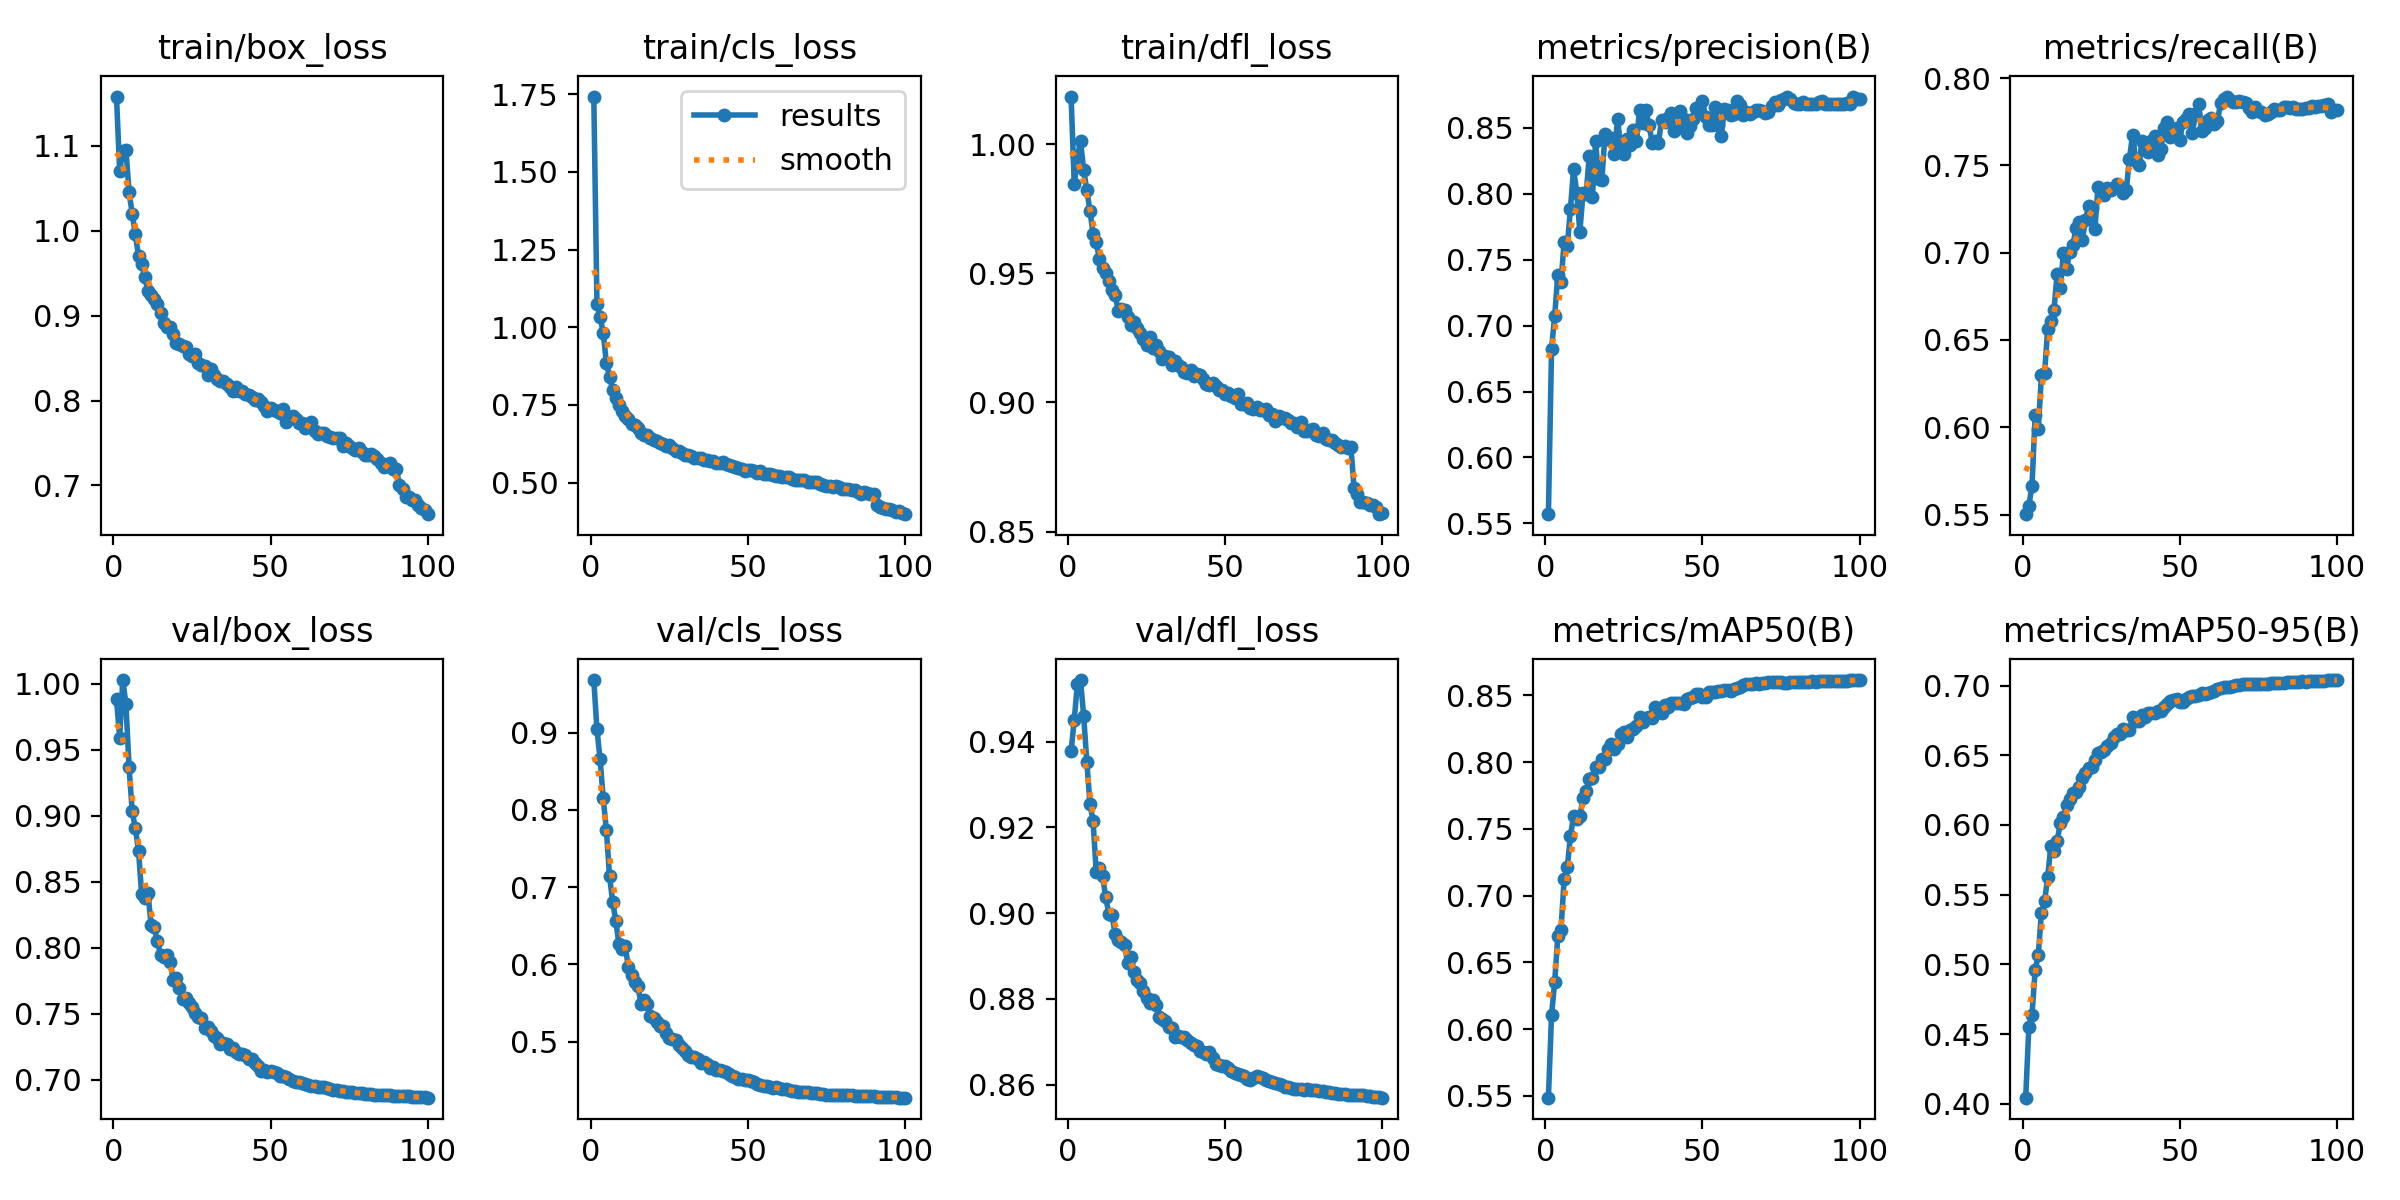
\includegraphics[width=0.9\linewidth]{Figures/results.png}
        \caption{Đồ thị Loss và mAP - Model 1}
    \end{figure}

    \framebreak

    \textbf{Kết quả chi tiết theo từng lớp:}
    \begin{table}
        \centering
        \begin{tabular}{|l|c|c|c|}
            \hline
            \textbf{Lớp} & \textbf{mAP@50} & \textbf{Precision} & \textbf{Recall} \\
            \hline
            Ô tô & \textbf{0.922} & 0.91 & 0.85 \\
            \hline
            Xe buýt & 0.897 & 0.88 & 0.80 \\
            \hline
            Xe máy & 0.872 & 0.85 & 0.79 \\
            \hline
            Xe tải & 0.832 & 0.84 & 0.75 \\
            \hline
            Xe đạp & 0.782 & 0.78 & 0.72 \\
            \hline
        \end{tabular}
    \end{table}

    \framebreak

    \begin{figure}
        \centering
        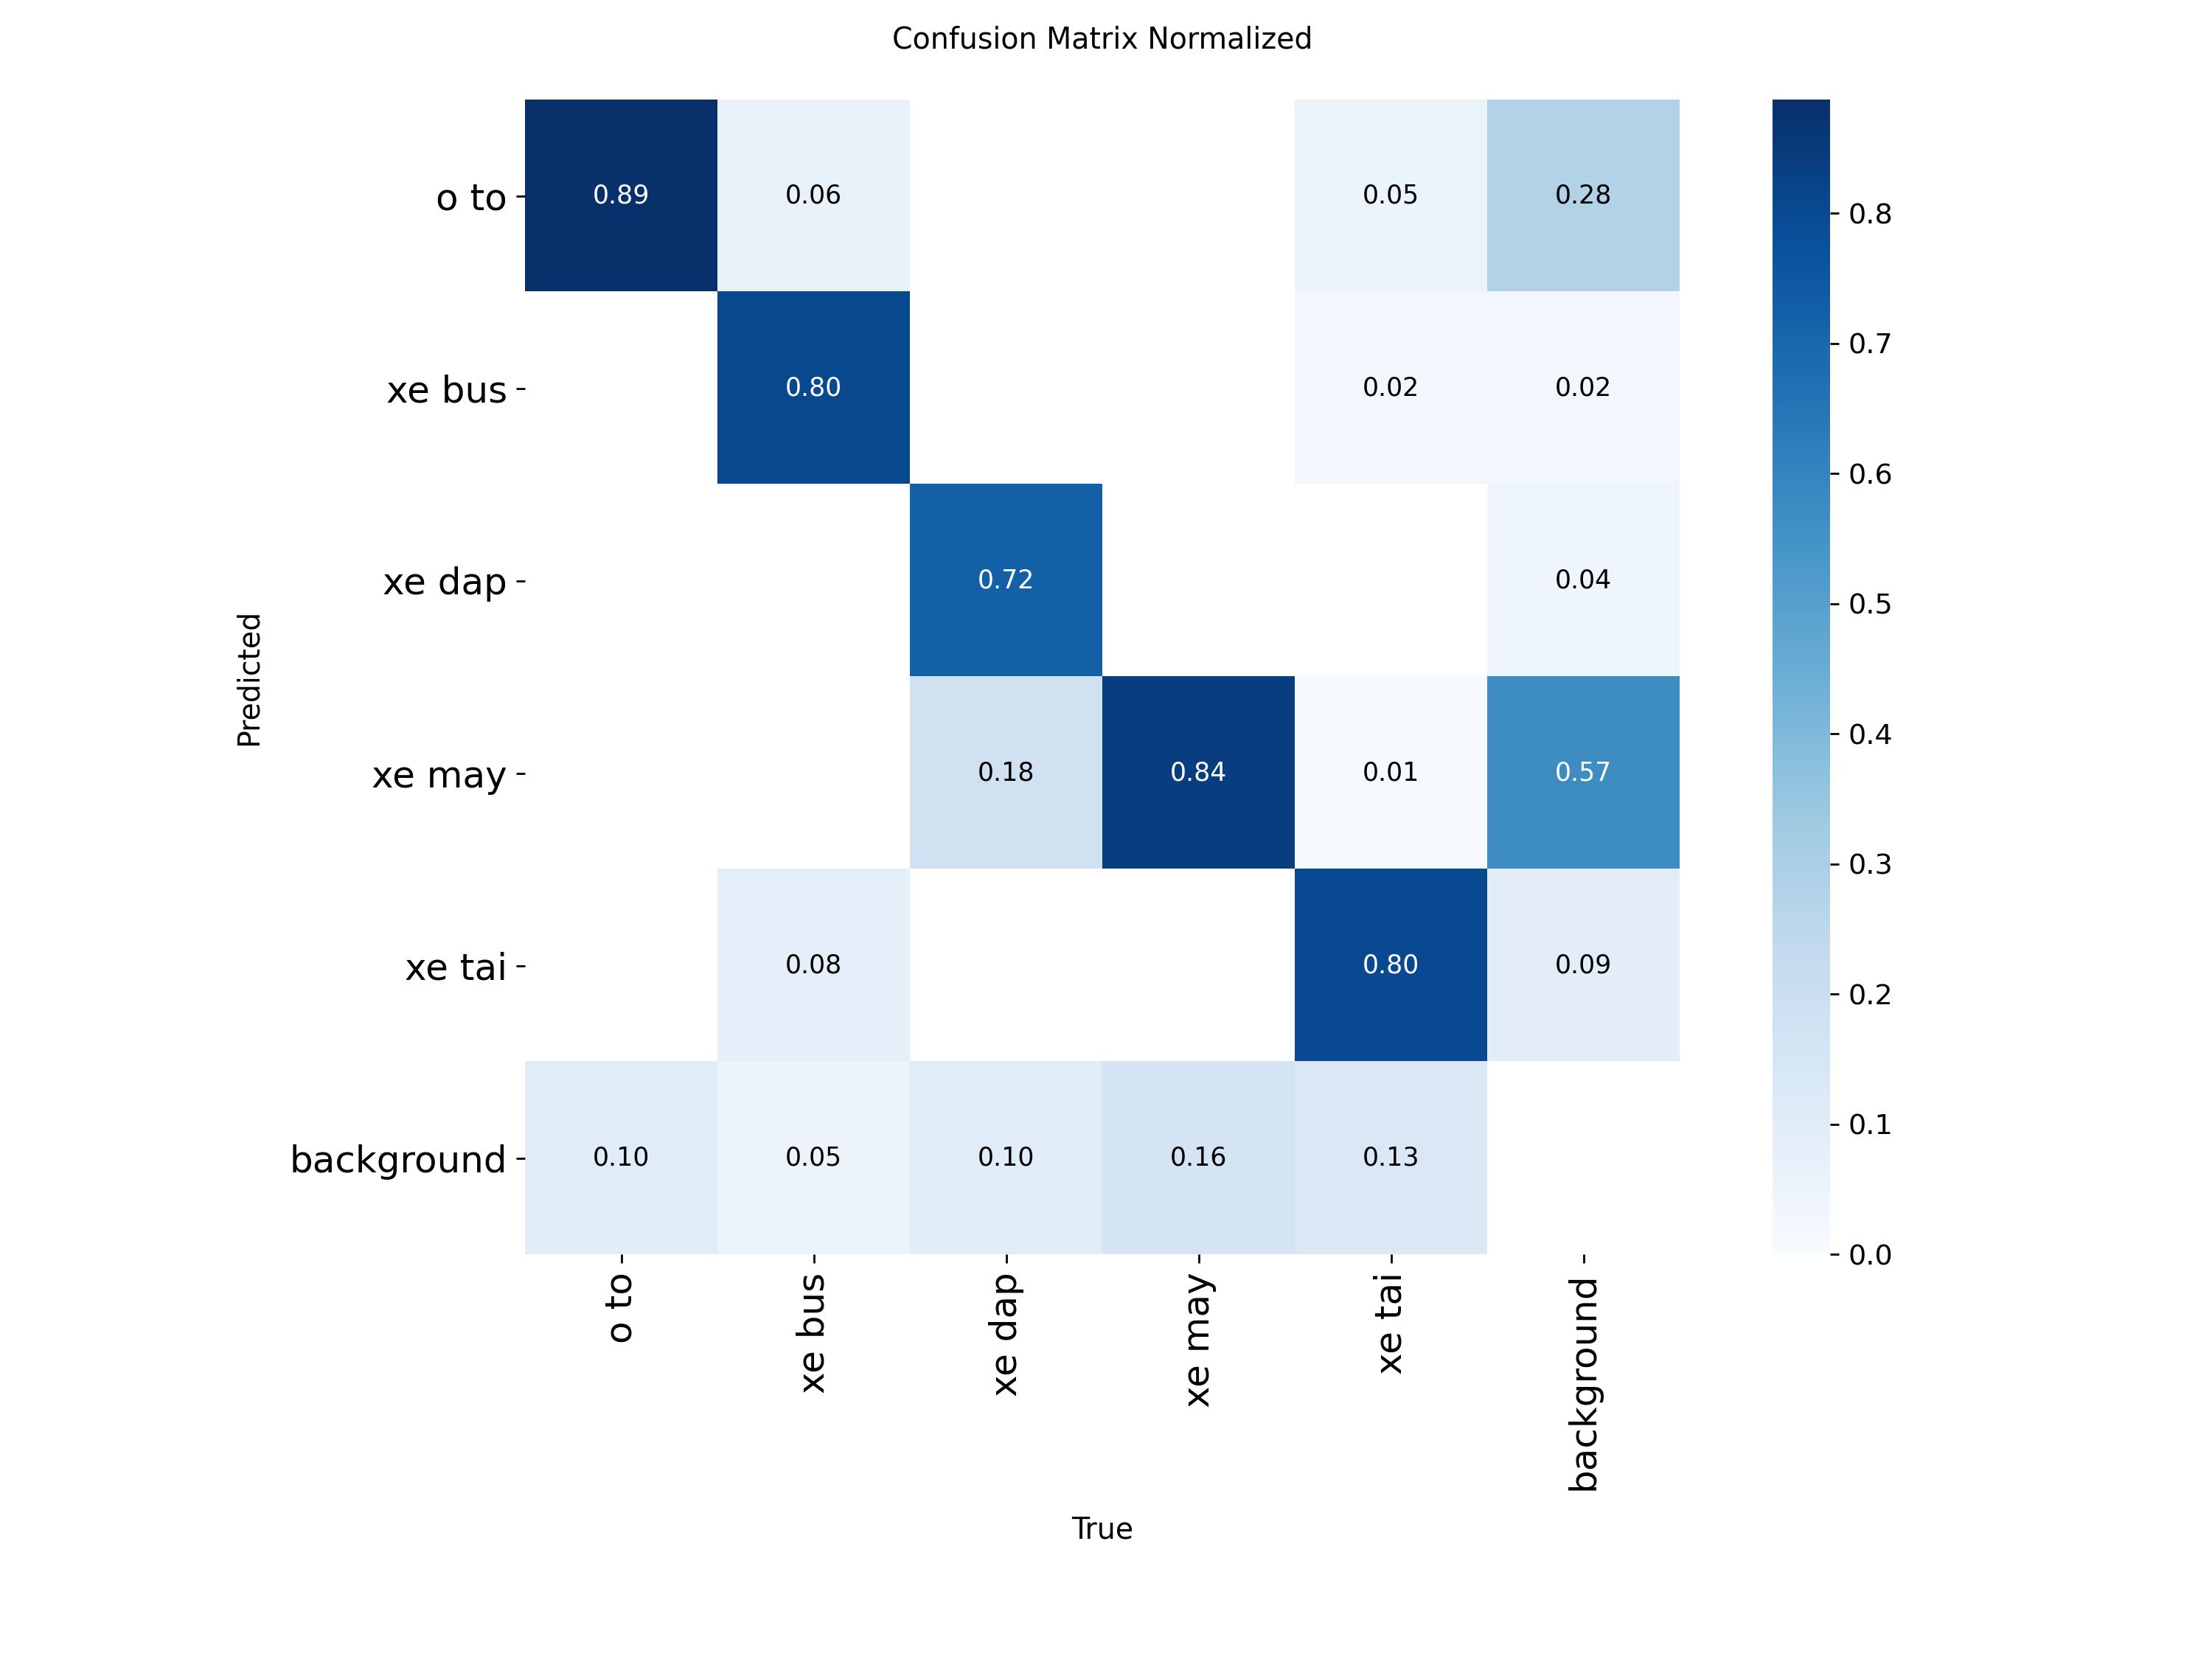
\includegraphics[width=0.65\linewidth]{Figures/confusion_matrix_normalized.png}
        \caption{Ma trận nhầm lẫn Model 1}
    \end{figure}

    \textbf{Nhận xét:} Nhầm lẫn chủ yếu giữa xe đạp và xe máy (18\%)
\end{frame}

%--- KẾT QUẢ MODEL 2 ---
\begin{frame}[allowframebreaks]{Kết quả Model 2: Phát hiện biển số}
    \begin{figure}
        \centering
        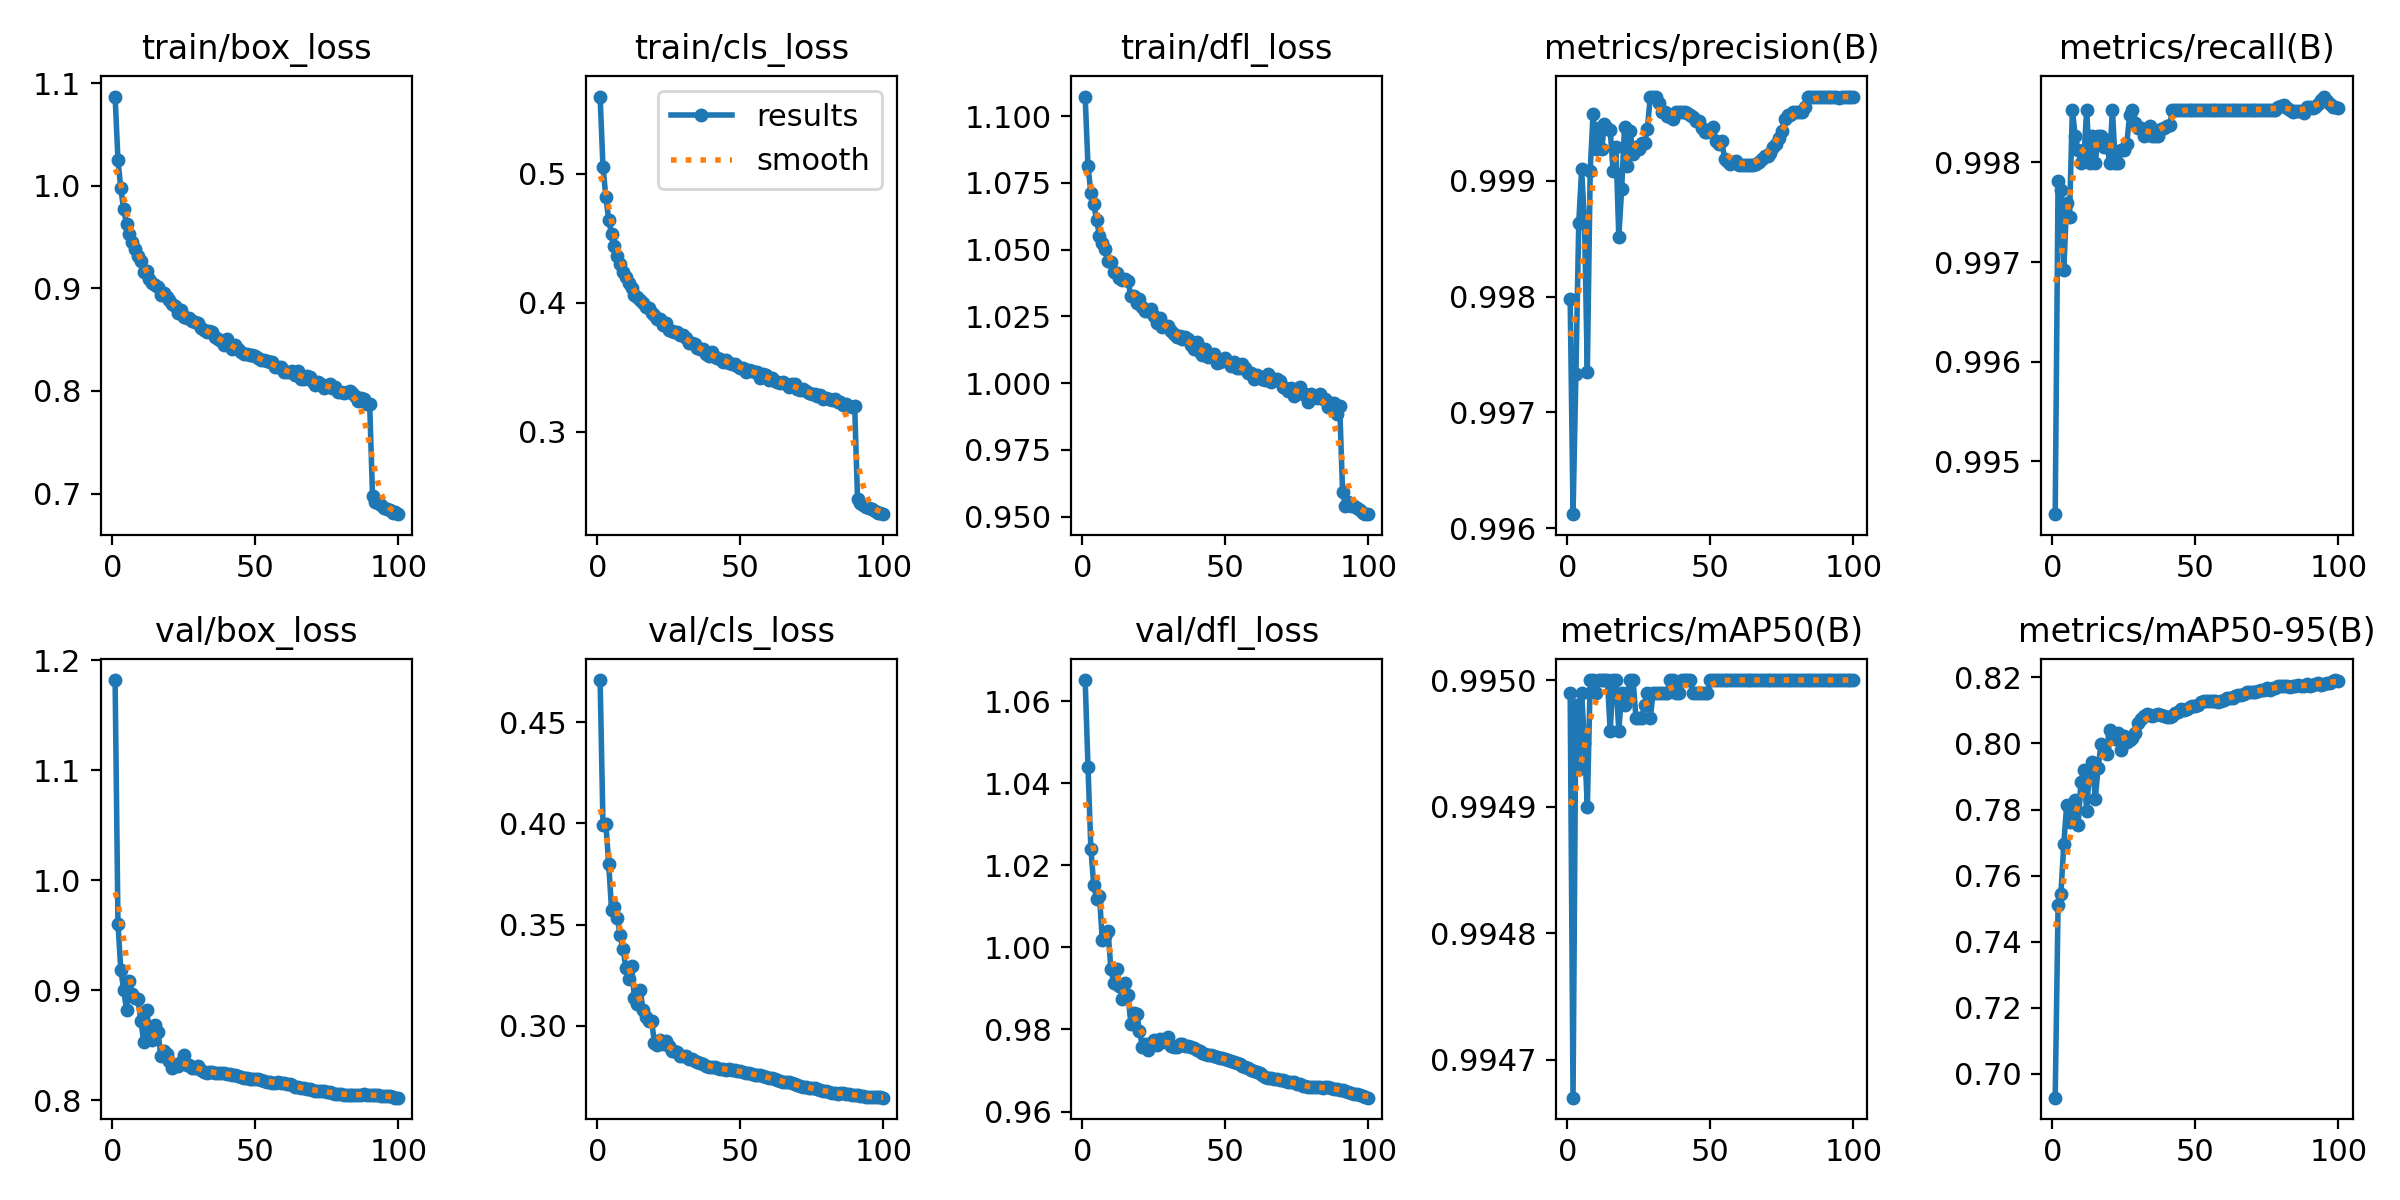
\includegraphics[width=0.9\linewidth]{Figures/plate_results.png}
        \caption{Đồ thị Loss và mAP - Model 2 (Plate Detection)}
    \end{figure}

    \framebreak

    \begin{alertblock}{Kết quả xuất sắc}
    \begin{itemize}
        \item \textbf{Precision:} 99.97\%
        \item \textbf{Recall:} 99.86\%
        \item \textbf{mAP@50:} 99.50\%
        \item \textbf{mAP@50-95:} 81.90\%
    \end{itemize}
    \end{alertblock}

    \textbf{Lý do đạt kết quả cao:}
    \begin{itemize}
        \item Bài toán phát hiện 1 lớp (single-class)
        \item Pretrained weights chất lượng
        \item Dataset VNLP đa dạng, được gán nhãn cẩn thận
    \end{itemize}

    \framebreak

    \begin{figure}
        \centering
        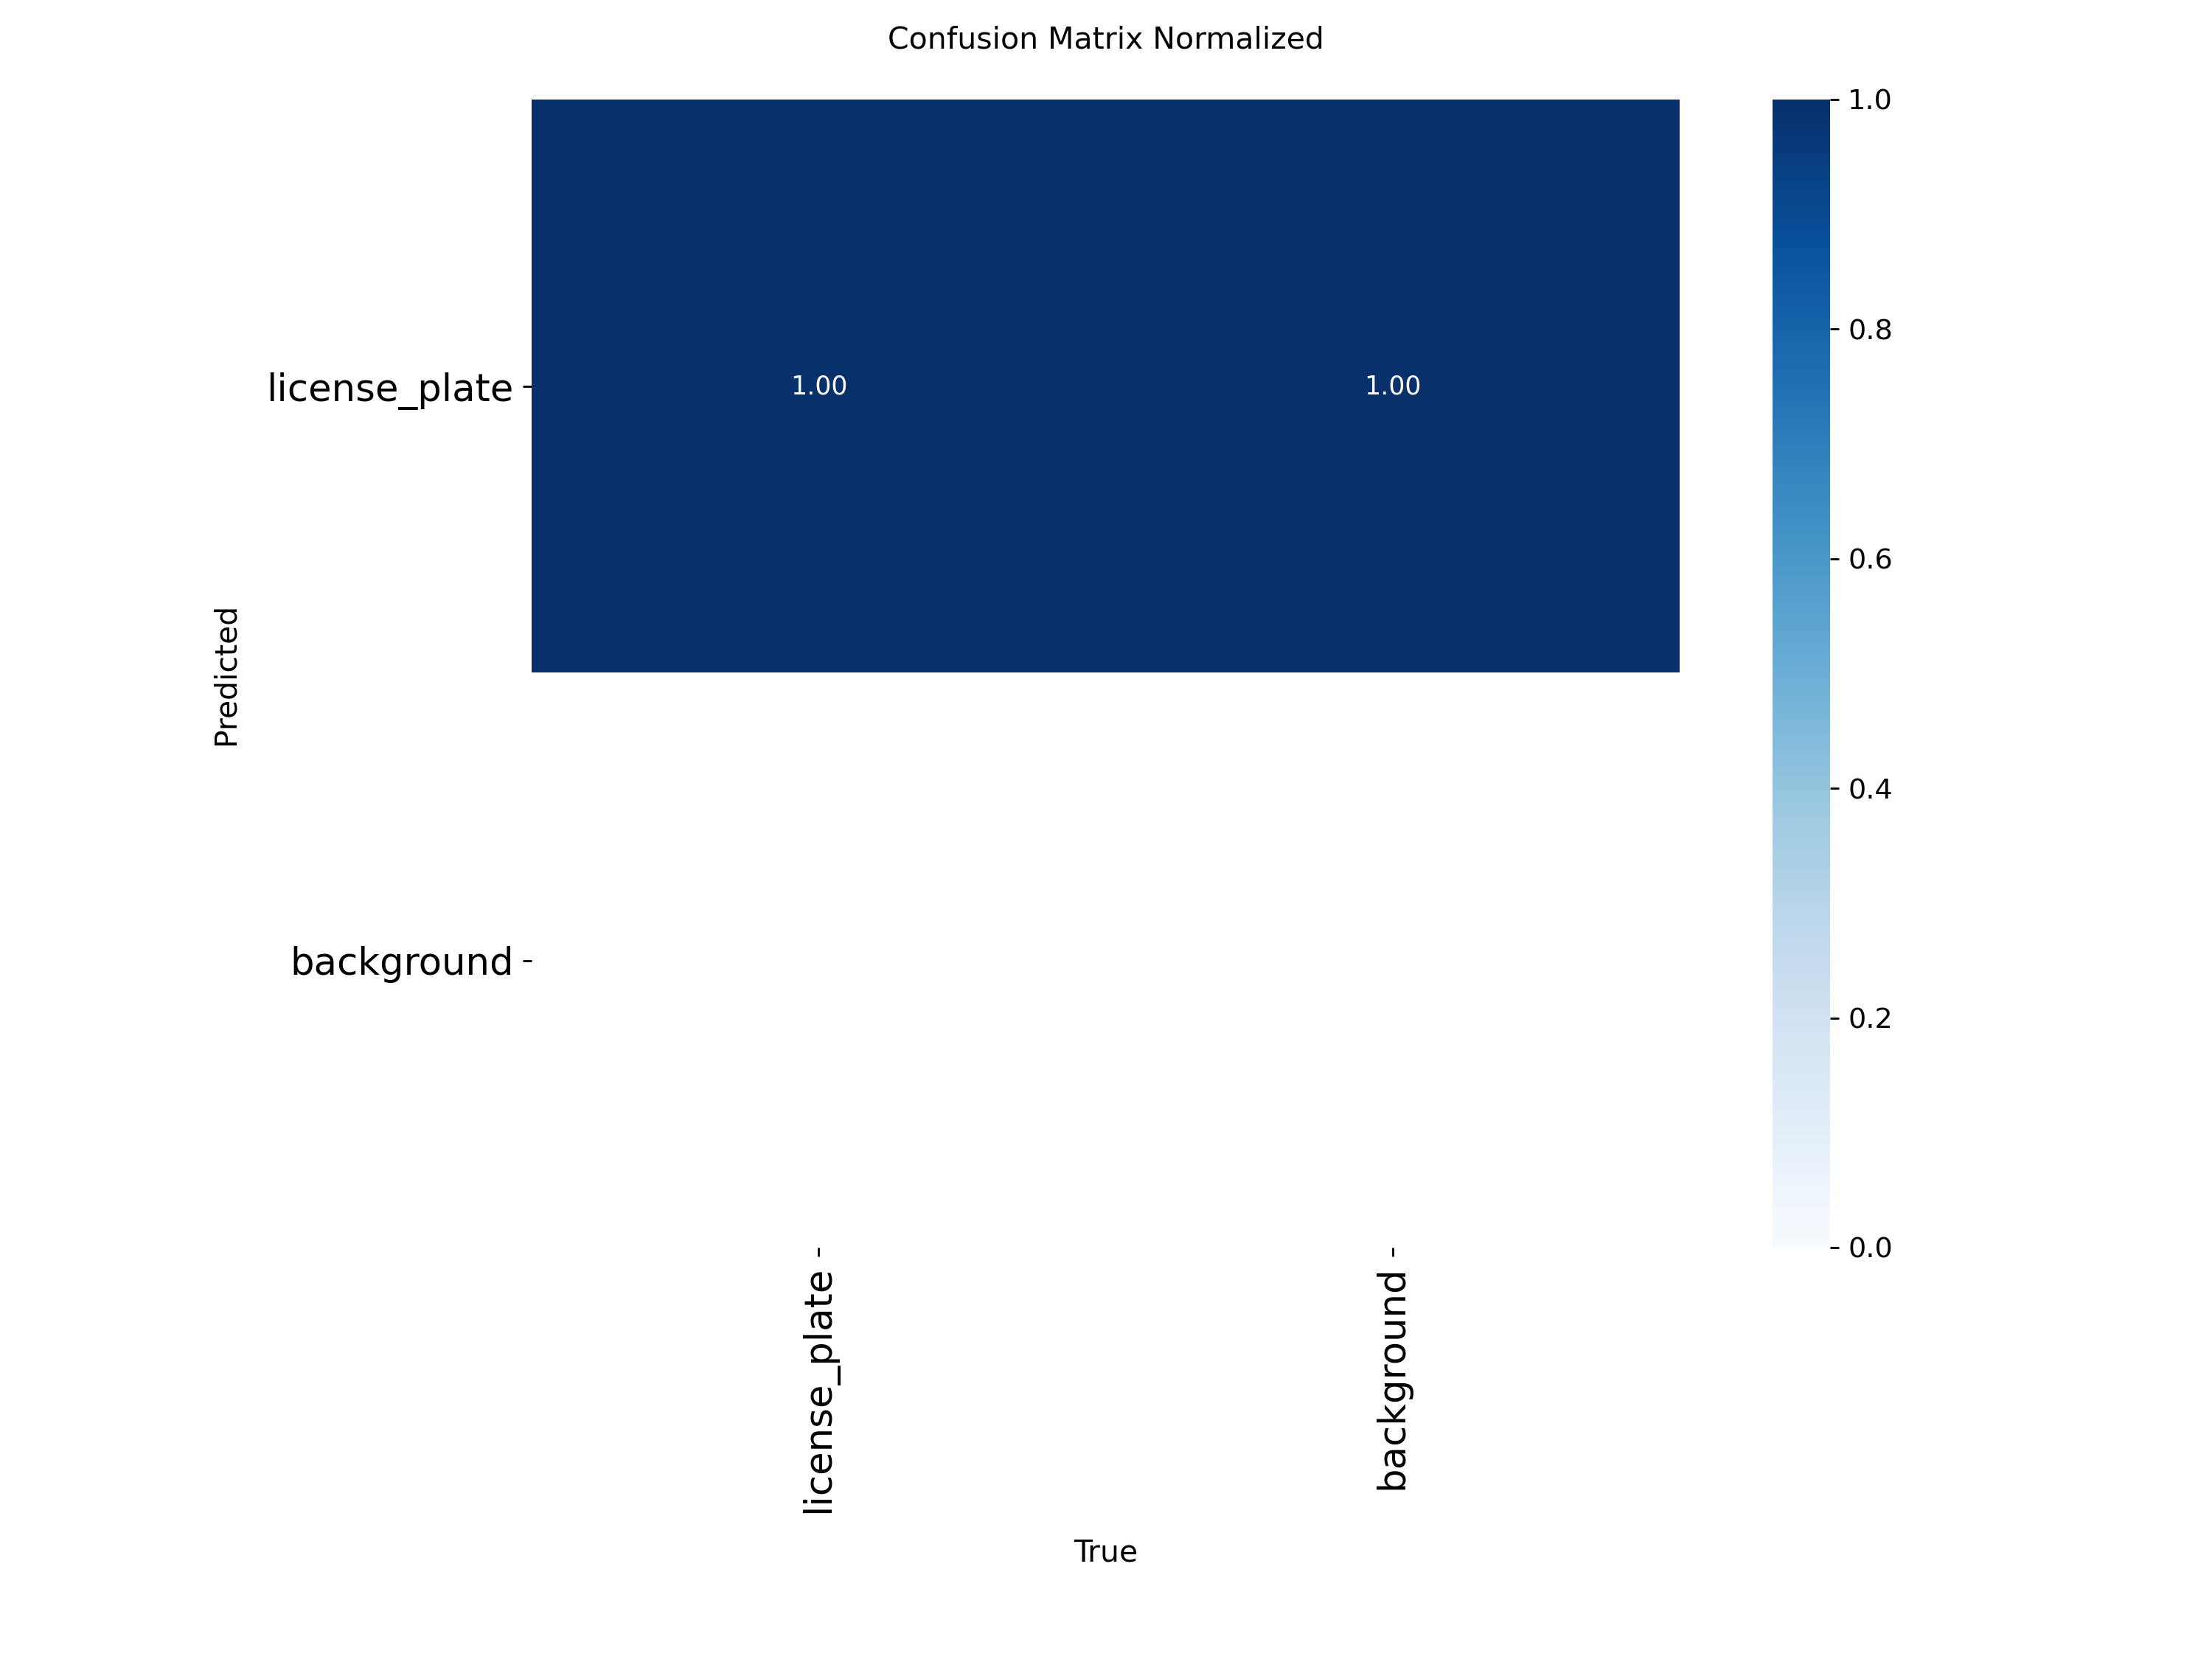
\includegraphics[width=0.55\linewidth]{Figures/plate_confusion_matrix.png}
        \caption{Ma trận nhầm lẫn Model 2 - Gần như hoàn hảo}
    \end{figure}
\end{frame}

%--- KẾT QUẢ MODEL TÍCH HỢP ---
\begin{frame}[allowframebreaks]{Kết quả Mô hình tích hợp 6 lớp}
    \begin{figure}
        \centering
        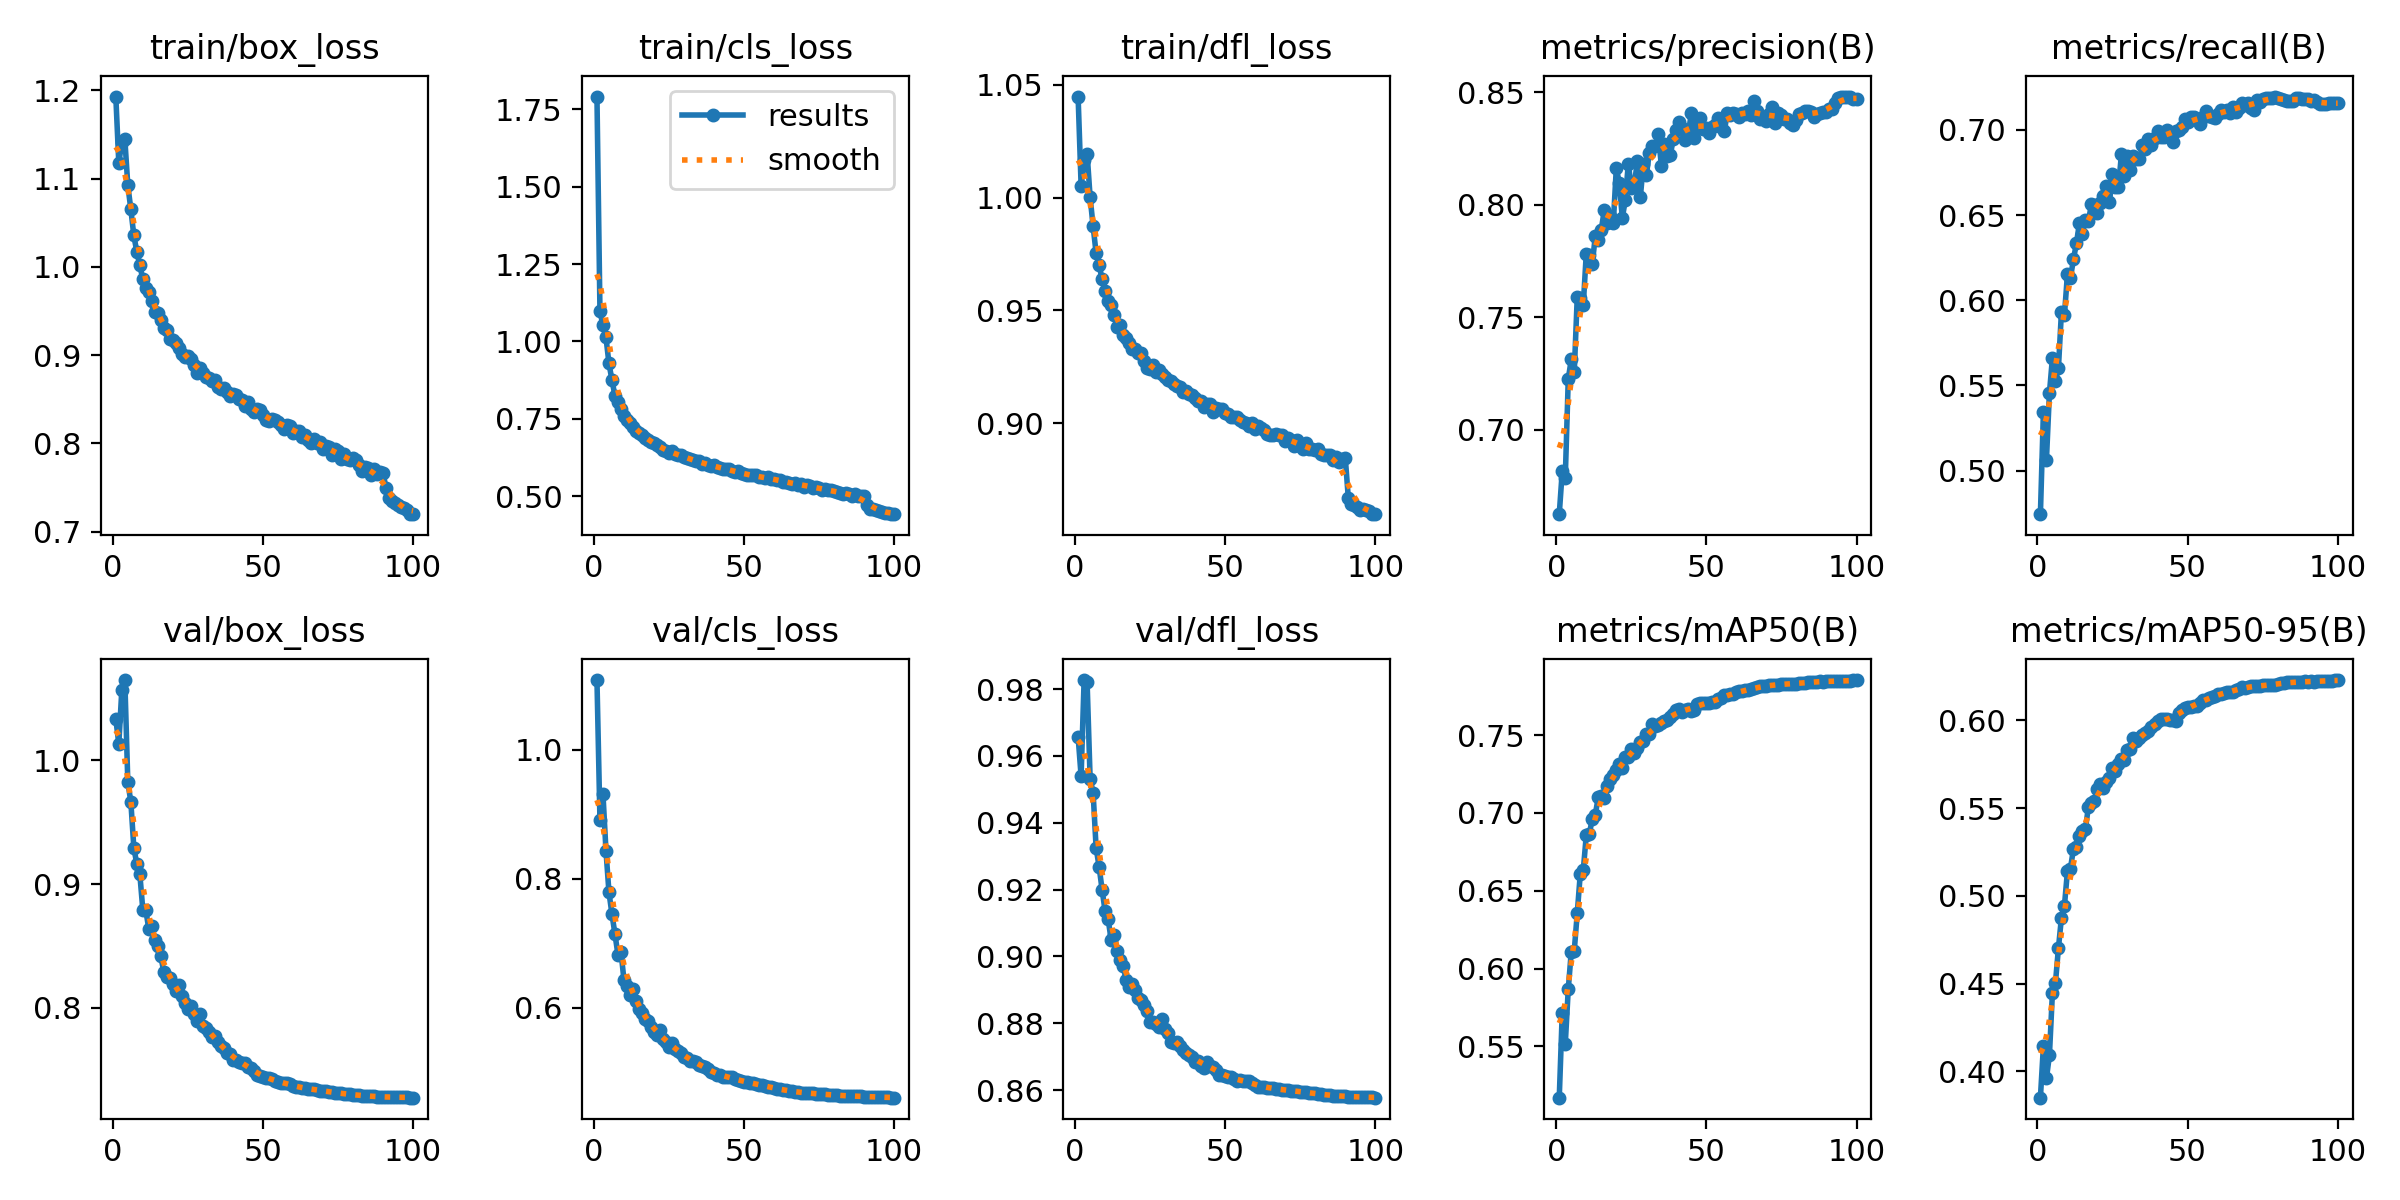
\includegraphics[width=0.9\linewidth]{Figures/multiclass_results.png}
        \caption{Đồ thị Loss và mAP - Mô hình tích hợp}
    \end{figure}

    \framebreak

    \textbf{Kết quả theo từng lớp:}
    \begin{table}
        \centering
        \begin{tabular}{|l|c|c|c|}
            \hline
            \textbf{Lớp} & \textbf{mAP@50} & \textbf{Precision} & \textbf{Recall} \\
            \hline
            Ô tô & 0.89 & 0.88 & 0.82 \\
            \hline
            Xe buýt & 0.86 & 0.85 & 0.78 \\
            \hline
            Xe máy & 0.84 & 0.83 & 0.76 \\
            \hline
            Xe tải & 0.81 & 0.82 & 0.73 \\
            \hline
            Xe đạp & 0.72 & 0.75 & 0.65 \\
            \hline
            \textbf{Biển số} & \textbf{0.59} & 0.72 & 0.56 \\
            \hline
        \end{tabular}
    \end{table}

    \textbf{Hạn chế:} Lớp biển số có mAP thấp (0.59) do class imbalance và kích thước nhỏ
\end{frame}

%--- KẾT QUẢ INFERENCE PIPELINE 2 ---
\begin{frame}[allowframebreaks]{Kết quả Inference Pipeline 2 (One-Stage)}
    \begin{figure}
        \centering
        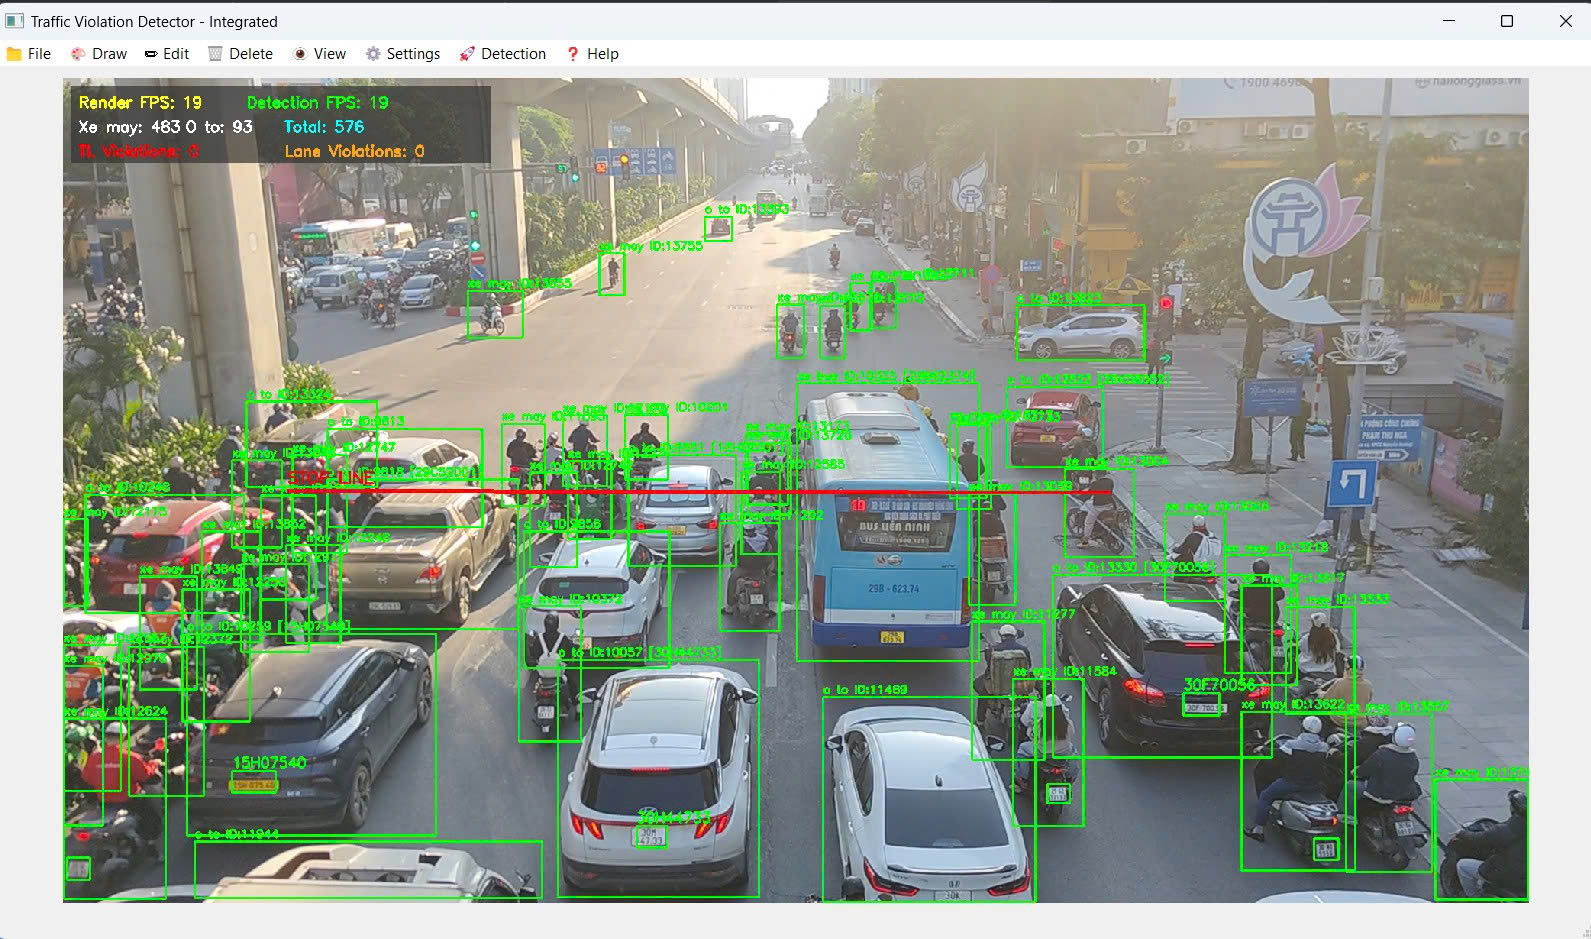
\includegraphics[width=0.85\linewidth]{Figures/ppthucnghiem2.jpg}
        \caption{Pipeline 2: Phát hiện đồng thời xe và biển số (1 model)}
    \end{figure}

    \framebreak

    \textbf{Ưu điểm quan sát được:}
    \begin{itemize}
        \item Phát hiện tốt các loại phương tiện với bbox chính xác
        \item Biển số được phát hiện khi có kích thước đủ lớn
        \item Mapping plate$\rightarrow$xe tự động qua containment check (95\% thành công)
    \end{itemize}

    \textbf{Hạn chế:}
    \begin{itemize}
        \item Biển số nhỏ/xa có thể bị bỏ sót
        \item Trade-off: Tốc độ nhanh nhưng mAP plate giảm
    \end{itemize}
\end{frame}

%--- SO SÁNH PIPELINE ---
\begin{frame}{So sánh hiệu năng hai Pipeline ALPR}
    \begin{table}
        \centering
        \small
        \begin{tabular}{|l|c|c|}
            \hline
            \textbf{Tiêu chí} & \textbf{Pipeline 1} & \textbf{Pipeline 2} \\
            & \textbf{(Two-Stage)} & \textbf{(One-Stage)} \\
            \hline
            FPS trung bình & 5--10 FPS & 15--20 FPS \\
            \hline
            mAP@50 (Plate) & \textbf{99.5\%} & 59\% \\
            \hline
            Số model cần load & 2 & 1 \\
            \hline
            GPU Memory & ~2.5GB & ~1.2GB \\
            \hline
            Phát hiện biển nhỏ & \textbf{Tốt} & Trung bình \\
            \hline
            Tài nguyên tiêu thụ & Cao & Thấp \\
            \hline
        \end{tabular}
        \caption{So sánh hai phương pháp ALPR (theo báo cáo)}
    \end{table}
\end{frame}

\begin{frame}{Khuyến nghị sử dụng}
    \begin{block}{Pipeline 1 (Two-Stage) - Ưu tiên độ chính xác}
    \begin{itemize}
        \item Yêu cầu độ chính xác cao cho biển số
        \item Camera có độ phân giải tốt
        \item Biển số nhỏ hoặc ở xa
    \end{itemize}
    \end{block}

    \begin{block}{Pipeline 2 (One-Stage) - Ưu tiên tốc độ}
    \begin{itemize}
        \item Yêu cầu xử lý real-time
        \item Tài nguyên phần cứng hạn chế
        \item Biển số đủ lớn trong khung hình
    \end{itemize}
    \end{block}
\end{frame}

%--- ĐÁNH GIÁ BYTETRACK ---
\begin{frame}{Đánh giá ByteTrack Tracking}
    \begin{block}{Kết quả thực tế}
    \begin{itemize}
        \item \textbf{ID Switch Rate:} < 5\% trên video thử nghiệm
        \item \textbf{Overhead:} ~2ms mỗi frame
        \item \textbf{Tính năng:} Kalman Filter + Hungarian Matching
    \end{itemize}
    \end{block}

    \begin{block}{Quan sát thực tế}
    \begin{itemize}
        \item \textbf{Hoạt động tốt:} Xe di chuyển bình thường, mật độ cao
        \item \textbf{ID switch xảy ra khi:}
        \begin{itemize}
            \item Xe bị che khuất > 2 giây
            \item Thay đổi tốc độ đột ngột
            \item Xe quá gần nhau (occlusion)
        \end{itemize}
    \end{itemize}
    \end{block}

    \textit{Cải thiện tiềm năng: Kết hợp Re-ID features}
\end{frame}

%--- ĐÁNH GIÁ OCR ---
\begin{frame}{Đánh giá OCR (PaddleOCR)}
    \begin{block}{Hiệu quả Format Validation}
    \begin{itemize}
        \item Loại bỏ kết quả nhiễu ngay từ đầu
        \item Chỉ hiển thị biển số đúng format VN
        \item Tận dụng tracking để retry tự động
    \end{itemize}
    \end{block}

    \textbf{Các trường hợp khó:}
    \begin{enumerate}
        \item Biển số bẩn/mờ: CLAHE giúp cải thiện nhưng hạn chế
        \item Góc nghiêng lớn: Perspective distortion giảm độ chính xác
        \item Ban đêm: Phản sáng từ đèn flash làm mất chi tiết
        \item Biển nhỏ/xa: Độ phân giải thấp
    \end{enumerate}
\end{frame}
